\chapter{Planning}

\paragraph{Seconda parte del corso:}

\begin{itemize}
  \item Comprendere i problemi fondamentali alla base degli algoritmi di pianificazione. 
  \item Studiare alcuni degli approcci classici alla pianificazione:
    \begin{itemize}
      \item Assunzioni del planning classico. 
      \item Algoritmi di ricerca nello spazio degli stati (progression, regression, STRIPS). 
      \item Algoritmi di ricerca nello spazio dei piani (least-commitment planning). 
      \item Algoritmi di ricerca basati su grafi (grafo di pianificazione, GRAPHLAN). 
      \item Euristiche domain-independent per il planning. 
      \item Altri approcci al planning (HTN).
    \end{itemize}
  \item Sistemi a regole:
    \begin{itemize}
      \item Paradigma dei sistemi esperti basati su regole di produzione. 
      \item Sperimentare il paradigma a regole in CLIPS.
    \end{itemize}
  \item Incertezza: 
    \begin{itemize}
      \item Modellare l'incertezza con le probabilità. 
      \item Meccanismi di inferenze probabilistiche.
    \end{itemize}
\end{itemize}

\section{Che Cos'è il Planning?}

\dfn{Planning (secondo Haslum)}{
  Il \newfancyglitter{planning} è l'arte e la pratica di pensare prima di agire.
}

\dfn{Automated Planning (Hoffman)}{
Selezionare un goal che motivi delle azioni basate su una descrizione ad alto livello del mondo.
}

\paragraph{In altre parole:}

\begin{itemize}
  \item Il planning è un processo deliberativo che sceglie ed organizza le azioni in base
all’effetto che ci si aspetta queste producano. 
\item AI planning è lo studio della calcolabilità di questo processo deliberativo.
\end{itemize}

\subsection{Modello Concettuale per il Planning}

\fancyglitter{State Transition System} $\Sigma = (S, A, E, \gamma)$
\begin{itemize}
    \item Dove:
    \begin{itemize}
        \item $S = \{s_1, s_2, \ldots\}$ insieme finito, ricorsivamente enumerabile di stati
        \item $A = \{a_1, a_2, \ldots\}$ insieme finito, ricorsivamente enumerabile di azioni
        \item $E = \{e_1, e_2, \ldots\}$ insieme finito, ricorsivamente enumerabile di eventi
        \item $\gamma : S \times (A \cup E) \rightarrow 2^S$ è una relazione di transizione di stato
    \end{itemize}
    
    \item Se $a \in A$ e $\gamma(s, a) \neq \emptyset$, allora $a$ è \fancyglitter{applicabile} in $s$
    
    \item Applicare $a$ in $s$ causerà una transizione di stato del sistema da $s$ a $s'$, dove $s' \in \gamma(s, a)$
\end{itemize}

\clm{}{}{
  Un STS $\Sigma = (S, A, E, \gamma)$ può essere rappresentato come un grafo diretto $G = (N_G, E_G)$ dove:
    \begin{itemize}
        \item $N_G = S$ è l’insieme dei nodi del grafo coincidente con l’insieme degli stati di $\Sigma$
        \item $E_G$ è l’insieme degli archi del grafo tale che esiste un arco $s \xrightarrow{u} s'$ (anche rappresentato come $\langle s, u, s' \rangle$) da $s$ a $s'$ etichettato con $u \in A \cup E$, \fancyglitter{se e solo se}:
        \begin{itemize}
            \item $s, s' \in S$ e
            \item $s' = \gamma(s, u)$
        \end{itemize}
    \end{itemize}
}

\begin{figure}[h]
    \centering
    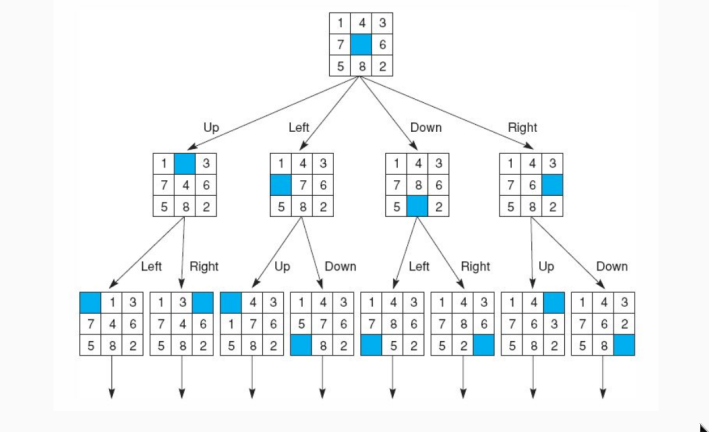
\includegraphics[scale=0.55]{01/sts.png}
    \caption{STS visto come grafo.}
\end{figure}

\paragraph{Ingredienti del planning:}

\begin{itemize}
  \item \fancyglitter{STS}: 
    \begin{itemize}
      \item Descrive tutte le possibili evoluzioni del sistema. 
    \end{itemize}
  \item \fancyglitter{Piano}:
    \begin{itemize}
      \item Struttura che traccia le azioni necessarie per raggiungere un certo obiettivo $G$ dato uno stato iniziale $I$. 
      \item È un cammino da $I$ a $G$ nello spazio degli stati tracciato da STS.  
    \end{itemize}
  \item \fancyglitter{Goals}:
    \begin{itemize}
      \item Un goal state $s_g$ o un sottoinsieme di possibili goal state $S_g$. 
      \item Soddisfacimento di condizioni in tutta la sequenza di stati prodotta dalle azioni. 
      \item Ottimizzazione di funzioni di utilità. 
      \item Vincoli sulle azioni che possono essere eseguite.
    \end{itemize}
\end{itemize}

\begin{minipage}{0.4\textwidth}
    \centering
    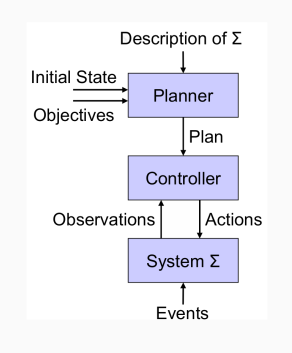
\includegraphics[width=\linewidth]{01/plan.png}
    \captionof{figure}{Si assume che gli eventi non interferiscano con il controller.}
\end{minipage}
\hfill
\begin{minipage}{0.5\textwidth}
    \begin{itemize}
        \item \fancyglitter{Planner:}
        \begin{itemize}
            \item Data la descrizione di un STS $\Sigma$, lo stato iniziale, e il goal.
            \item Genera un piano che raggiunge il goal dallo stato iniziale.
        \end{itemize}

        \item \fancyglitter{Controller:}
        \begin{itemize}
            \item Dato un piano e lo stato corrente (funzione di osservabilità $\eta : S \rightarrow O$).
            \item Seleziona ed esegue un’azione del piano.
        \end{itemize}

        \item \fancyglitter{STS $\Sigma$:}
        \begin{itemize}
            \item Evolve in funzione delle azioni eseguite e degli eventi che possono accadere.
        \end{itemize}
    \end{itemize}
\end{minipage}


\begin{minipage}{0.4\textwidth}
    \centering
    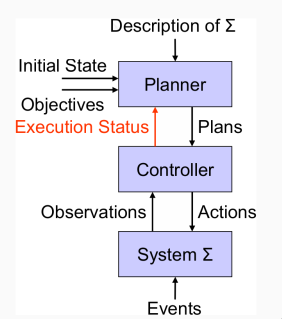
\includegraphics[width=\linewidth]{01/stsc.png}
    \captionof{figure}{Gli eventi possono interferire.}
\end{minipage}
\hfill
\begin{minipage}{0.5\textwidth}
    \begin{itemize}
        \item \fancyglitter{Challenge:}
        \begin{itemize}
            \item Il mondo reale può essere diverso da come è descritto nel modello.
        \end{itemize}
        \item \fancyglitter{Continual planning:}
        \begin{itemize}
            \item Plan supervision.
            \item Plan revision.
            \item Re-planning.
        \end{itemize}

        \item Continual planning consente un loop chiuso di feedback tra planner e controller.
    \end{itemize}
\end{minipage}

\subsection{Pianificazione Classica}

\nt{La pianificazione classica è la pianificazione che avviene sotto alcune assunzioni.}

\dfn{Dominio Finito}{
$\Sigma$ contiene un numero finito di stati.
}

\cor{Rilassare un Dominio Finito (A0)}{
  Per: 
  \begin{itemize}
    \item Descrivere azioni che producono nuovi oggetti nel mondo. 
    \item Trattare fluenti numerici. 
  \end{itemize}
  Problemi:
  \begin{itemize}
    \item Decidibilità e terminazione del pianificatore.
  \end{itemize}
}

\dfn{Dominio Completamente Osservabile}{
  La funzione $\eta: S \rightarrow O$ è la funzione identità.
}

\cor{Rilassare un Dominio Completamente Osservabile (A1)}{
Per 
\begin{itemize}
  \item Trattare state in cui non tutto è osservabile o può essere conosciuto.
\end{itemize}
Problemi:
\begin{itemize}
  \item In genere si osserva solo un sottoinsieme della realtà, può accadere che $\eta(s) = \eta(s') = o$ con $s \not= s'$.
  \item Le osservazioni sono ambigue perché consistenti con più stati possibili. 
  \item Determinare lo stato successore può essere problematico. 
    \item Conformant planning (pianificazione in assenza di osservazioni): pianificare a prescindere dal reale stato del mondo.
\end{itemize}

}

\dfn{Dominio Deterministico}{
$\Sigma$ è deterministico, cioè per ogni $s \in S, u \in A \cup E$ si ha $|\gamma (s, u)| \leq 1$.
}

\cor{Rilassare un Dominio Deterministico (A2)}{
Per: 
\begin{itemize}
  \item Pianificare con azioni che possono avere risultati alternativi.
\end{itemize}
Problemi:
\begin{itemize}
  \item Il controller deve osservare il risultato reale di ogni azione. 
  \item Il piano soluzione potrebbe contenere dei branch condizionali o iterativi.
\end{itemize}
}

\dfn{Dominio Statico}{
$\Sigma$ è statico, ovvero $E = \emptyset$ e STS può essere ridotto a $\Sigma = (S, A, \gamma)$.
}

\cor{Rilassare un Dominio Statico (A3)}{
Per: 
\begin{itemize}
  \item Modellare domini in cui eventi al di là del controllo dell'esecutore sono possibili.
\end{itemize}
Problemi:
\begin{itemize}
  \item Il mondo diventa non deterministico dal punto di vista del pianificare.
\end{itemize}
}

\dfn{Dominio con Goal Semplici}{
Consistono in uno stato $s_g$ da raggiungere o un insieme di stati $S_g$ (è sufficiente che il piano porti a uno di essi). 
}

\nt{Gli stati possono essere descrizioni parziali di situazioni desiderate.}

\cor{Rilassare un Dominio con Goal Semplici (A4)}{
Per:
\begin{itemize}
  \item Trattare vincoli su stati e piani, funzioni di utilità/costo, ottimalità.
\end{itemize}
Problemi:
\begin{itemize}
  \item Esprimere e ragionare su vincoli ulteriori nella specifica del goal rende il planning computazionalmente costoso.
\end{itemize}

}

\dfn{Dominio con Piani Sequenziali}{
 Un piano soluzione è una sequenza finita di azioni linearmente ordinate. 
}

\nt{Una sola azione per volta è possibile.}

\cor{Rilassare un Dominio con Piani Sequenziali (A5)}{
Per: 
\begin{itemize}
  \item Sfruttare le capacità degli esecutori nel caso potessero eseguire più azioni. 
  \item Non introdurre vincoli che non sono parte del dominio.
\end{itemize}
Problemi: 
\begin{itemize}
  \item Ragionare su e gestire strutture dati più complesse.
\end{itemize}
}

\dfn{Dominio con Tempo Implicito}{
Le azioni e gli eventi non hanno durata (oppure hanno durata istantanea).
}

\cor{Rilassare un Dominio con Tempo Implicito (A6)}{
Per: 
\begin{itemize}
  \item Trattare azioni durative, problemi di concorrenza e deadline.
\end{itemize}
Problemi:
\begin{itemize}
  \item Rappresentare e ragionare sul tempo. 
  \item Gli effetti delle azioni si sviluppano nel tempo.
\end{itemize}
}

\dfn{Dominio con Single Agent}{
  Un solo pianificatore e un solo controller (esecutore).
}

\cor{Rilassare un Dominio con Single Agent (A7)}{
Per:
\begin{itemize}
  \item Sfruttare meglio le risorse disponibili. 
  \item Trattare situazioni in cui più esecutori sono presenti ma non sono sotto il controller di un unico pianificatore.
\end{itemize}
Problemi:
\begin{itemize}
  \item Multi-agent planning: necessità di trattare le interazioni, coordinazione, competizione, negoziazione e planning della teoria dei giochi.
\end{itemize}
}

\subsection{Problemi di Pianificazione Classica}

\paragraph{Un problema di pianificazione classica è $P = (\Sigma, s_0, S_g)$:}

\begin{itemize}
  \item $\Sigma = (S, A, \gamma)$ è il modello del dominio espresso come STS. 
  \item $s_0 \in S$ è lo stato iniziale. 
  \item $S_g \subset S$ è l'insieme degli stati goal.
\end{itemize}

\paragraph{Una soluzione $\pi$ a un problema $P$:}

\begin{itemize}
  \item Una sequenza totalmente ordinata di azioni istanziate (ground). $\pi = \langle a_1, a_2, \dots, a_n \rangle$.
  \item Danno origine a una sequenza di transazioni di stato  $\langle s_0, s_1, \dots, a_n \rangle$ tale che:
    \begin{itemize}
      \item $s_1 = \gamma(s_0, a_1)$. 
      \item $\forall k: 2..n s_k = \gamma(s_{k-1}, a_k)$. 
      \item $s_n \in S_g$.
    \end{itemize}
\end{itemize}

\qs{}{Quali sono le sfide dell'approccio classico al planning?}

\begin{itemize}
  \item Come rappresentare stati e azioni in modo da non dover
esplicitamente enumerare S, A, e $\gamma$?
\item Come ricercare una soluzione in modo efficiente? Quali algoritmi? Quali euristiche?
\item Come generalizzare le soluzioni? Classical Planning troppo semplice per essere utile nei casi pratici, ma può essere la base per soluzioni in contesti più complessi (rilassando alcune assunzioni).
\end{itemize}

\qs{}{Perché la pianificazione è difficile?}

\begin{itemize}
  \item È dimostrabile che il planning è un task computazionalmente costoso:
    \begin{itemize}
      \item \fancyglitter{PlanSAT}: esiste un piano che risolve un problema di pianificazione? 
      \item \fancyglitter{Bounded PlanSAT}: esiste un piano di lunghezza k? 
    \end{itemize}
  \item Per la pianificazione classica entrambi i problemi sono decidibili (la
ricerca avviene in spazio finito). 
\item Se si estende a uno spazio infinito: 
  \begin{itemize}
    \item PlanSAT diventa semi-decidibile: esiste un algoritmo che termina quando la soluzione non esiste, potrebbe non terminare quando la soluzione non esiste.
    \item Bounded PlanSAT rimane decidibile.
  \end{itemize}
\end{itemize}

\clm{}{}{
  \begin{itemize}
    \item Bounded PlanSAT è NP completo mentre PlanSAT è P. 
    \item Trovare una soluzione è meno costoso che trovare una soluzione ottima. 
    \item La complessità del planning giustifica la ricerca di euristiche, possibilmente domain-independent, che guidino il pianificatore nella sintesi di una soluzione.
  \end{itemize}
}

\paragraph{Proprietà di un buon algoritmo di pianificazione:}

\begin{itemize}
  \item \fancyglitter{Soundness} (correttezza): un pianificatore è corretto se tutte le soluzioni che trova sono piani corretti, ovvero realmente eseguibili dal controller: 
    \begin{itemize}
      \item Tutti i goals sono soddisfatti. 
      \item Nessuna precondizione di azione è open (mancante). 
      \item Nessun vincolo ulteriore è violato (vincoli temporali, istanziazione di variabili, etc.). 
    \end{itemize}
  \item \fancyglitter{Completeness} (completezza): 
    \begin{itemize}
      \item Un pianificatore è completo se trova una soluzione quando il problema è risolubile. 
      \item Un pianificatore è strettamente completo se tutte le soluzioni sono mantenute nello spazio di ricerca (eventuali \textit{pruning} dello spazio non scartano soluzioni).
    \end{itemize}
  \item \fancyglitter{Ottimalità}: un pianificatore è ottimo se l'ordine con cui le soluzioni sono trovate è coerente con una qualche misura di qualità dei piani (lunghezza, costo complessivo, etc.).
\end{itemize}

\nt{Molti algoritmi, per favorire la velocità, rinunciano all'ottimalità.}

\section{Algoritmi di Pianificazione}

\subsection{Ricerca in Avanti e Ricerca all'Indietro}

\dfn{Progression}{
Calcolo dello stato successore $s'$ di uno stato $s$ rispetto all'applicazione di un operatore $o$:
$$s' = \gamma(s, o)$$

}

\paragraph{Pianificatori basati su progression applicano delle ricerche in avanti tipicamente nello spazio degli stati:}

\begin{itemize}
  \item La ricerca comincia da uno stato iniziale. 
  \item Iterativamente viene applicato un operatore $o$ per generare un nuovo stato $s'$. 
  \item La soluzione è trovata quando lo stato $s'$ appena generato soddisfa il goal ($s' \vDash s_g$ e $s_g \in S_g$).
  \item Ha il vantaggio di essere molto intuitivo e facile da implementare.
\end{itemize}

\begin{figure}[h]
    \centering
    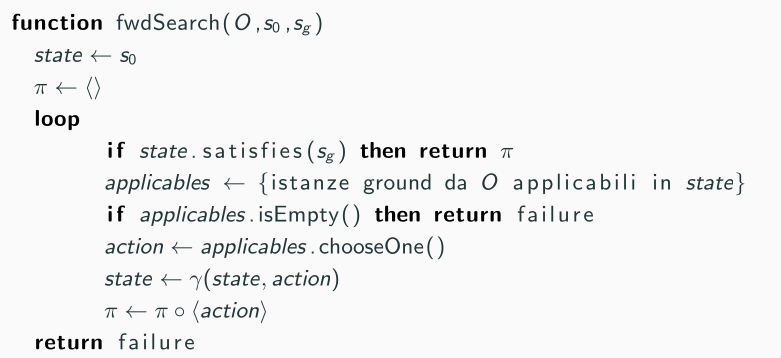
\includegraphics[scale=0.4]{01/progression.png}
    \caption{applicables.chooseOne() rappresenta una scelta non deterministica, ma esaustiva, di un'azione.}
\end{figure}

\nt{chooseOne() avrà varie implementazioni a seconda dell'algoritmo scelto.}

\cor{Soundness di Progression}{
  fwdSearch è corretto: se la funzione termina con un piano come soluzione, allora questo piano è effettivamente una soluzione al problema iniziale.
}

\cor{Completeness di Progression}{
fwdSearch è completo: se esiste una soluzione allora esiste una traccia d'esecuzione che restituirà quella soluzione come piano.
}

\clm{}{}{
  \begin{itemize}
    \item Il numero di azioni applicabili in un dato stato è in genere molto grande. 
    \item Anche il branching factor tende a essere grande. 
    \item La ricerca in avanti corre il rischio di non essere praticabile dopo pochi passi.    
  \end{itemize}

}

\paragraph{Ricerca in avanti vs. Ricerca all'indietro:}

\begin{itemize}
  \item La ricerca in avanti comincia da un singolo stato iniziale mentre la ricerca all'indietro comincia da un insieme di stati. 
  \item Quando si applica in avanti un operatore $o$ a uno stato $s$ si genera un unico stato successore $s'$, all'indietro possono esserci molteplici stati predecessori. 
  \item Nella ricerca in avanti lo spazio di ricerca coincide con lo spazio degli stati, all'indietro ogni stato dello spazio di ricerca corrisponde a un insieme di stati del dominio.
\end{itemize}

\dfn{Regression}{
Il calcolo del regresso, ovvero il sottogoal predecessore di un goal dato, avviene nel seguente modo:
\begin{itemize}
  \item Dato un goal $g$. 
  \item Sia $a$ azione ground tale che $g \in effects^+(a)$.
  \item $g' = \gamma^{-1} (g, a) = (g \ effects^+(a)) \cup pre(a)$.
\end{itemize}
$g'$ è il regresso di $g$ attraverso la relazione di transizione $\gamma$ e l'azione $a$.
}

\paragraph{Nella ricerca all'indietro:}

\begin{itemize}
  \item Si comincia dall'insieme di stati goal. 
  \item Iterativamente si seleziona un sottogoal generato precedentemente e si regredisce attraverso un operatore generando un nuovo sottogoal. 
  \item La soluzione è trovata quando il nuovo sottogoal è soddisfatto dallo stato iniziale. 
  \item Ha il vantaggio di poter gestire più stati contemporaneamente. 
  \item È più costoso e difficile.
\end{itemize}

\begin{figure}[h]
    \centering
    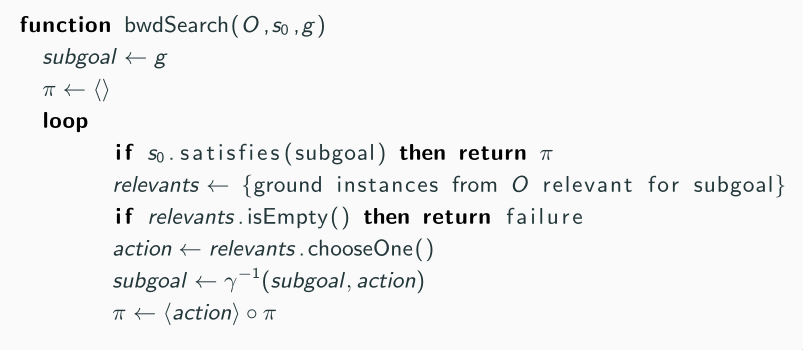
\includegraphics[scale=0.4]{01/regression.png}
\end{figure}

\clm{}{}{
  \begin{itemize}
    \item La ricerca all'indietro si basa su azioni rilevanti, cioè quelle che contribuiscono attivamente al goal: 
      \begin{itemize}
        \item Producono almeno uno degli atomi che compaiono nel goal. 
        \item Non hanno effetti negativi sul goal stesso (non negano uno degli atomi del goal).
      \end{itemize}
    \item La ricerca all'indietro mantiene un fattore di ramificazione più basso rispetto alla ricerca in avanti, ma il fatto di dover mantenere un belief state può complicare le strutture dati usate dal planner e la definizione di euristiche. 
    \item Nonostante il vantaggio teorico la ricerca in avanti è preferita alla ricerca all'indietro.
  \end{itemize}
}

\subsection{STRIPS}

\dfn{STRIPS}{
  STanford Research Institute Problem Solver: 
  \begin{itemize}
    \item Introduce una rappresentazione esplicita degli operatori di pianificazione. 
    \item Fornisce una operalizzazione delle nozioni di:
      \begin{itemize}
        \item Differenza tra stati. 
        \item Subgoal. 
        \item Applicazione di un operatore. 
      \end{itemize}
    \item Gestisce il Frame Problem. 
    \item Si basa su due idee fondamentali: 
      \begin{itemize}
        \item Linear planning. 
        \item Means-End Analysis.
      \end{itemize}
  \end{itemize}
}
\clm{Linear Planning}{}{
  \begin{itemize}
    \item Idea di base: 
      \begin{itemize}
        \item Risolvere un goal per volta, passare al successivo solo quando il precedente è stato raggiunto. 
      \end{itemize}
    \item L'algoritmo di planning mantiene uno \fancyglitter{stack dei goal}: 
      \begin{itemize}
        \item Risolvere un goal può comportare la risoluzione di sottogoal. 
      \end{itemize}
    \item Conseguenze:
      \begin{itemize}
        \item Non c'è interleaving nel conseguimento dei goal. 
        \item La ricerca è efficiente se i goal non interferiscono troppo tra loro. 
        \item Ma è soggetto alla \fancyglitter{Sussmann's Anomaly}. 
      \end{itemize}
  \end{itemize}
}

\begin{figure}[h]
    \centering
    
\includegraphics[scale=0.1]{01/susman.jpg}
    \caption{Sussmann's Anomaly caught in 4k.}
\end{figure}

\clm{Means-End Analysis}{}{
  \begin{itemize}
    \item Idea di base:
      \begin{itemize}
        \item Considera solamente gli aspetti rilevanti al problema (backward). 
        \item Quali mezzi (means, operatori) sono disponibili e necessari per raggiungere il goal (end).
      \end{itemize}
    \item Occorre stabilire quali differenze ci sono tra lo stato corrente e il goal. 
    \item Trovare un operatore che riduce tale differenza. 
    \item Ripetere l'analisi sui sottogoal ottenuti per regressione attraverso l'operatore selezionato.
  \end{itemize}
}

\paragraph{Caratteristiche di STRIPS:}

\begin{itemize}
  \item È un sottoinsieme della logica del primordine: 
    \begin{itemize}
      \item Numero finito di simboli di predicati, simboli di costanti e senza simboli di funzione né quantificatori.
    \end{itemize}
  \item Uno stato in STRIPS è una congiunzione di \fancyglitter{atomi ground} (privi di simboli di funzione). 
  \item Vige l'\fancyglitter{assunzione di mondo chiuso}: quello che non è descritto è considerato falso.
  \item Semantica degli insiemi:
    \begin{itemize}
      \item Un atomo ground $p$ vale in uno stato $s$ se e solo se $p \in s$. 
    \end{itemize}
  \item Semantica logic-oriented: 
    \begin{itemize}
      \item Uno stato $s$ soddisfa una congiunzione di letterali $g$, denotato come $s \vDash g$ se ogni letterale positivo in $g$ occorre in $s$ e se ogni letterale negativo in $g$ non occorre in $s$. 
    \end{itemize}
\end{itemize}

\paragraph{Relazioni Fluenti:}

\begin{itemize}
  \item Predicati che rappresentano relazioni il cui valore di verità può cambiare da uno stato al successivo. 
\end{itemize}

\paragraph{Relazioni Persistenti:}

\begin{itemize}
  \item Predicati il cui valore di verità non può cambiare.
\end{itemize}

\dfn{Plan Operators}{
  Un operatore di pianificazione in STRIPS è una tripla: $o: (name(0), precond(o), effects(o))$ dove:
  \begin{itemize}
    \item $name(o)$ è una rappresentazione sintattica del tipo $n(x_1,\dots, x_k)$ dove $n$ è il nome dell'operatore e $x_1, \dots, x_k$ è una lista di variabili che compaiono in $o$. 
    \item $precond(o)$ è l'insieme di letterali che rappresentano le precondizioni dell'azione. 
    \item $effect(o)$ è l'insieme di letterali che rappresentano gli effetti dell'azione. 
  \end{itemize}
}

\nt{Una variabile può comparire negli effetti solo se è anche menzionata nelle precondizioni.}

\dfn{Calcolo dello Stato Successore (progression)}{
  Sia $s$ uno stato del mondo ($s \in S$ per un dato dominio $\Sigma$). Sia $a$ un'azione. Diremo che $a$ è \newfancyglitter{applicabile} in $s$ se e solo se: 
  \begin{itemize}
    \item $precond^+(a) \subseteq s$. 
    \item $precond^-(a) \cap s = \emptyset$.
  \end{itemize}
La funzione di transizione di stato $\gamma(s, a)$ è definita:
\begin{itemize}
  \item Se $a$ è applicabile in $s$:
    \begin{itemize}
      \item $\gamma(s, a) = (s \ effects^-(a)) \cup effects^+(a)$. 
      \item Altrimenti $\gamma(s, a)$ è indefinita.
    \end{itemize}
\end{itemize}
}

\nt{STRIPS usa la progression per modificare lo stato corrente a cui si giunge eseguendo le azioni fin qui selezionate nel piano in costruzione.}

\dfn{Calcolo del Sottogoal Predecessore (regression)}{

  Il calcolo del regresso avviene:
  \begin{itemize}
    \item Dato un goal $g$. 
    \item Sia $a$ azione ground tale che $g \in effects^+$(a). 
    \item $g' = \gamma^{-1}(g, a) = (g \ effects^+(a)) \cup pre(a)$
  \end{itemize}
  
}

\nt{STRIPS usa la regression per ridurre la distanza tra il goal che si vuole raggiungere e lo stato corrente.}

\begin{figure}[h]
    \centering
    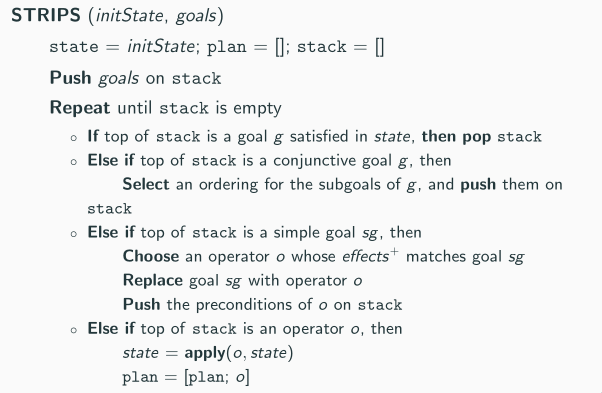
\includegraphics[scale=0.6]{01/strips.png}
\end{figure}

\paragraph{Il planner di STRIPS:}

\begin{itemize}
   \item[\textcolor{green}{\ding{51}}] Lo spazio di ricerca è ridotto perché i goal sono considerati uno per volta. 
      \item[\textcolor{green}{\ding{51}}] Ideale quando i goal sono indipendenti tra loro. 
         \item[\textcolor{green}{\ding{51}}] È sound. 
      \item[\textcolor{red}{\ding{55}}] Può produrre piani subotttimi (Sussmann's Anomaly). 
         \item[\textcolor{red}{\ding{55}}] È incompleto (perché alcune azioni in alcuni domini non sono reversibili).
\end{itemize}

\dfn{Sussmann's Anomaly}{
  È necessario disfare parte dei goal già raggiunti per poter risolvere l'intero problema.
}

\nt{È una conseguenza di:
\begin{itemize}
  \item Interdipendenza tra i sottogoal. 
  \item Ordinamento sfavorevole dei goal.
\end{itemize}
}

\dfn{Planning Domain Definition Language}{
  PDDL è uno standard per definire problemi e domini. Nella sua versione base è una sistematizzazione di STRIPS.
}

\paragraph{Estensioni di PDDL:}

\begin{itemize}
  \item \fancyglitter{Conditional effects}: stabilire che alcuni effetti sono raggiunti solo se sono vere certe condizioni. 
  \item \fancyglitter{Durative actions}: un plan operator si divide in tre parti: 
    \begin{itemize}
      \item Un evento iniziale. 
      \item Un evento finale. 
      \item Una condizione invariante che deve permanere per tutta la durata dell'azione. 
    \end{itemize}
  \item \fancyglitter{Numeric fluent}: consente di tracciare il consumo di risorse nel tempo. 
  \item \fancyglitter{Quantificators}.
\end{itemize}

\section{Pianificazione nello Spazio dei Piani}

\qs{}{Come costruire un modello espresso da variabili di stato?}

\begin{itemize}
  \item Dato un ambiente $E$ che si vuole modellare. 
  \item Dato l'insieme degli oggetti \fancyglitter{rilevanti} $B$. 
  \item $B$ deve astrarre i dettagli insignificanti (non indispensabili per la risoluzione del problema).
\end{itemize}

\paragraph{Gli oggetti hanno due tipi di proprietà:}

\begin{itemize}
  \item \fancyglitter{Rigid}:
    \begin{itemize}
      \item Proprietà invarianti, persistono in ogni possibile stato del sistema. 
      \item Nella rappresentazione classica corrispondono agli atomi grounf. 
      \item In una rappresentazione state-variable questi atomi ground corrispondono a costanti booleane. 
    \end{itemize}
  \item \fancyglitter{Varying}: 
    \begin{itemize}
      \item Possono cambiare nelle transizioni di stato. 
      \item Nella rappresentazione classica solo le relazioni fluenti che vengono aggiunte/tolte per effetto delle azioni. 
      \item Sono modellate come variabili a cui possiamo assegnare un valore. 
      \item Uno stato è rappresentato su un insieme e ogni variabile di stato ha un dominio.
    \end{itemize}
\end{itemize}

\paragraph{Logica del primordine vs. state-variable:}

\begin{itemize}
  \item La logica del primordine ha origini storiche, il planning viene visto come meccanismo di theorem proving. 
  \item La logica del primordine è \fancyglitter{equivalente} a state-variable:
    \begin{itemize}
      \item Stesso potere espressivo. 
      \item Riconducibili l'uno all'altro. 
    \end{itemize}
  \item State-variable è più sintetica e uniforme. 
  \item State-variable si presta meglio a estensioni verso il non classical planning e all'uso di euristiche domain-independent.
\end{itemize}

\subsection{Least-Commitment Planning}

\dfn{Principio Least-Commitment}{
  Si fanno scelte solo quando sono indispensabili per risolvere una parte del problema e durante la ricerca non si pongono più vincoli dello stretto necessario.
}

\paragraph{Decisioni che è possibile ritardare:}

\begin{itemize}
  \item \fancyglitter{Ordinamenti}: non ordinare le azioni a meno che non sia strettamente necessario. 
  \item \fancyglitter{Bindings}: non ordinare le azioni a meno che non sia indispensabile unificarle con costanti al fine di conseguire i goal.
\end{itemize}

\paragraph{Idea:}

\begin{itemize}
  \item La ricerca avviene nello spazio dei piani. 
  \item Ogni nodo della ricerca è un piano parzialmente ordinato con \fancyglitter{flaws} (difetti). 
  \item A ogni passo si rimuove un difetto per mezzo di \fancyglitter{raffinamenti incrementali} del piano parziale corrente. 
  \item Se l'algoritmo termina con successo il piano risultante è completamente istanziato ma solo parzialmente ordinato.
\end{itemize}

\nt{Spazio di ricerca = insieme dei piani parziali.}

\paragraph{Un piano è una tupla $\langle A, O, B, L\rangle$ dove:}

\begin{itemize}
  \item $A$ è l'insieme di azioni, anche parzialmente istanziate. 
  \item $O$ è l'insieme dei \fancyglitter{vincoli di ordinamento} della forma $a_i < a_j$, è una rekazione d'ordine parzialmente definita. 
  \item $B$ è l'insieme dei \fancyglitter{bindings} (vincoli) della forma: 
      \begin{itemize}
        \item $v_i = C$, a $v_i$ è assegnata la costante $C$.
           \item $v_i \not= C$, $v_i$ può assumere qualsiasi valore tranne $C$.
              \item $v_i = v_j$, $v_i$ e $v_j$ assumono lo stesso valore.
                  \item $v_i \not= v_j$, $v_i$ e $v_j$ devono essere distinte.
      \end{itemize}
    \item $L$ è l'insieme di \fancyglitter{causal links} della forma $a_i \rightarrow^c a_j$, in cui $c$ è un effetto dell'azione $a_i$ che è necessario per l'azione $a_j$. 
\end{itemize}

\cor{Flaws - Open Goals}{
  Sia $\pi$ il piano del nodo corrente: 
  \begin{itemize}
    \item Una precondizione $p$ per un'azione $b$ è un open goal se non c'è un link causale a supporto di $p$. 
    \item Si può risolvere il difetto aggiungendo il link causale mancante:
      \begin{enumerate}
        \item Si trova un'azione $a$ tale che:
          \begin{itemize}
            \item $p$ può appartenere a $effect^+(a)$. 
            \item $a$ può precedere $b$ in $\pi$. 
          \end{itemize}
        \item Si istanzia l'azione $a$ in modo che asserisca $p$. 
        \item Si aggiunge un vincolo di precedenza tra $a$ e $b$ in $O$. 
        \item Si aggiunge un causal link $a \rightarrow^p b$ in $L$. 
      \end{enumerate}
  \end{itemize}
}

\cor{Flaws - Threats}{
 Sia $\pi$ il piano del nodo corrente:
 \begin{itemize}
  \item Dato un link causale $l: a \rightarrow^p b$. 
  \item Un'azione $c$ minaccia il link $l$ se: 
    \begin{itemize}
      \item $c$ può modificare il valore di verità di $p$ e può posizionarsi tra $a$ e $b$. 
      \item $c$ può produrre $p$, il link $l$ impone che sia $a$ a produrre $p$ e non un'altra azione $c$. 
    \end{itemize}
  \item $c$ viene detta \fancyglitter{clobber}.
 \end{itemize}

}

\paragraph{Risolvere le minacce:}

\begin{itemize}
  \item \fancyglitter{Promotion}: imporre il vincolo che $c$ precede $a$. 
  \item \fancyglitter{Demotion}: imporre il vincolo che $b$ precede $a$. 
  \item \fancyglitter{Separation}: imporre un vincolo di non-codesignation in modo tale che l'effetto di $c$ non unifichi con $p$.
\end{itemize}

\begin{figure}[h]
    \centering
    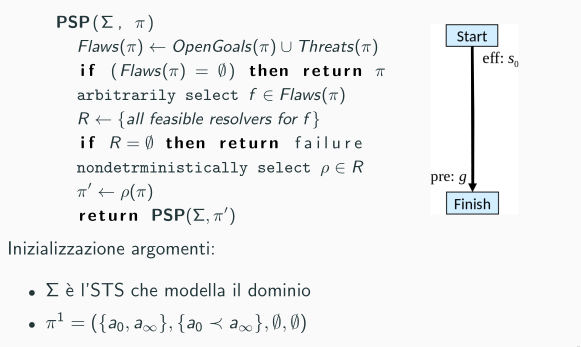
\includegraphics[scale=0.4]{01/psp.png}
    \caption{Algoritmo di Plan-Space Planning (PSP).}
\end{figure}

\clm{}{}{
PSP è corretto e completo: 
\begin{itemize}
  \item Ritorna un piano parzialmente ordinato $\pi$ tale che qualsiasi ordinamento totale delle sue azioni raggiunge il goal. 
  \item Dove il dominio lo consenta, le azioni non strettamente sequenziali possono essere eseguite in parallelo.
\end{itemize}
}

\section{Graphplan}

\subsection{Introduzione}

\dfn{Grafo di Pianificazione}{
  Struttura dati speciale per:
  \begin{itemize}
    \item Definire euristiche domain-independent. 
    \item Generare un piano.
  \end{itemize}
}

\nt{Il grafo astrae lo spazio di ricerca e può essere costruito con un algoritmo polinomiale.}

\paragraph{In dettaglio:}

\begin{itemize}
  \item Grafo orientato aciclico organizzato a livelli:
    \begin{itemize}
      \item Livello iniziale $S_0$ che contiene tutti i letterali che valgono nello stato iniziale (un nodo per ogni fluente). 
      \item Livello di azioni $A_0$ che contiene le azioni ground che possono essere applicate a $S_0$. 
      \item In generale $S_i, A_i$ si alternano fino a che non si raggiunge una condizione di terminazione: 
        \begin{itemize}
          \item $S_i$ contiene tutti i letterali che \fancyglitter{potrebbero} valere al tempo $i$. 
          \item $A_i$ contiene tutte le azioni che \fancyglitter{potrebbero} avere le precondizioni soddisfatte al tempo $i$.
        \end{itemize}
    \end{itemize}
\end{itemize}

\clm{}{}{
  \begin{itemize}
    \item Graphplan (GP) traccia solo un sottoinsieme delle possibili interazioni negative (un letterale che appare in uno stato $S_i$ per la prima volta) potrebbe di fatto essere producibile solo in uno stato successivo a $S_i$. Tuttavia $i$ è una buona stima per il letterale. 
      \item GP è costruito a partire da azioni ground. 
      \item Ogni $S_i$ è un \fancyglitter{belief state}: codifica più stati possibili e alternative. 
  \end{itemize}
}

\paragraph{Quando si costruisce il grafo bisogna tenere a mente che:}

\begin{itemize}
  \item Un letterale al tempo $i$ può essere inteso sia come precondizione di un'azione in $A_i$ sia come atomo persistente. In questo caso la persistenza è realizzata da un'azione speciale \texttt{no-op}. 
  \item In ogni livello $S_i$ possono essere presenti link di \fancyglitter{mutua esclusione} tra letterali. 
  \item In ogni livello $A_i$ possono essere presenti link di \fancyglitter{mutua esclusione} tra azioni. 
  \item GP cresce monotonicamente, quindi prima o poi si livella: due stati consecutivi $S_i$ e $S_{i + 1}$ sono identici. 
\end{itemize}

\paragraph{Mutua esclusione tra due azioni in un dato livello $A_i$:}

\begin{itemize}
  \item \fancyglitter{Effetti inconsistenti:} un'azione nega gli effetti dell'altra. 
  \item \fancyglitter{Interferenza:} uno degli effetti di un'azione è la negazione di una precondizione dell'altra. 
  \item \fancyglitter{Competizione delle precondizioni:} una delle precondizioni di un'azione è mutuamente esclusiva con le precondizioni dell'altra. 
\end{itemize}

\paragraph{Mutua esclusione tra due letterali in un dato livello $S_i$:}

\begin{itemize}
  \item \fancyglitter{Complementarity:} se uno è la negazione dell'altro. 
  \item \fancyglitter{Inconsistent Support:} se ogni possibile coppia di azioni al livello $A_{i - 1}$ che producono i due letterali sono mutuamente esclusive.
\end{itemize}

\qs{}{Perché la costruzione di un GP è polinomiale?}

\begin{itemize}
  \item I: letterali. 
  \item a: azioni. 
  \item Ogni livello $S_i$ ha non più di $I$ nodi e $I^2$ mutex tra letterali. 
  \item Ogni livello $A_i$ non ha più di $I + a$ nodi e $(a + I)^2$ link di mutex. 
  \item Un grafo con $n$ livelli ha dimensione $O(n(a + I)^2)$ e la stessa complessità per costruirlo. 
\end{itemize}

\clm{}{}{
  \begin{itemize}
    \item Se un letterale del goal non compare in nessun livello allora il goal non è raggiungibile. 
    \item Se anche tutti i letterali del goal compaiono in un qualche livello del GP non vuol dire che esista una soluzione. 
  \end{itemize}
}

\paragraph{Euristiche per stimare il costo di un singolo letterale:}

\begin{itemize}
  \item Profondità del livello tra quelli in cui un letterale del goal compare per la prima volta. 
    \item Lunghezza del piano serializzabile estratto dal GP.
\end{itemize}

\paragraph{Euristiche per stimare il costo di una congiunzione di letterali:}

\begin{itemize}
  \item \fancyglitter{Max-level:} prendere il massimo livello tra quelli in cui un letterale del goal compare per la prima volta. 
  \item \fancyglitter{Somma dei livelli:} assume indipendenza dei letterali del goal, non è ammissibile. 
  \item \fancyglitter{Livello di insieme:} profondità del livello in cui tutti i letterali del goal compaiono senza che alcuna coppia di essi sia in mutua esclusione: 
    \begin{itemize}
      \item È ammissibile, funziona bene quando i letterali sono indipendenti tra di loro. 
      \item Ignora le dipendenze tra tre o più letterali.
    \end{itemize}
\end{itemize}

\thm{}{
  Se esiste un piano valido allora questo è un sottografo del grafo di pianificazione. 
}

\paragraph{Intuitivamente:}

\begin{enumerate}
  \item Si espande il grafo un livello per volta fino a quando tutti gli atomi del goal non compaiono all'interno dell'$i$-esimo stato. 
  \item Si invoca \texttt{extract-solution} per cercare un piano all'interno del grafo: 
    \begin{itemize}
      \item Se trova una soluzione termina con successo. 
      \item Se la soluzione non esiste \fancyglitter{certamente} termina con insuccesso. 
      \item In tutti gli altri casi va al punto 3.
    \end{itemize}
  \item Si espande il grafo di un livello e si torna al passo 2.
\end{enumerate}

\begin{figure}[h]
    \centering
    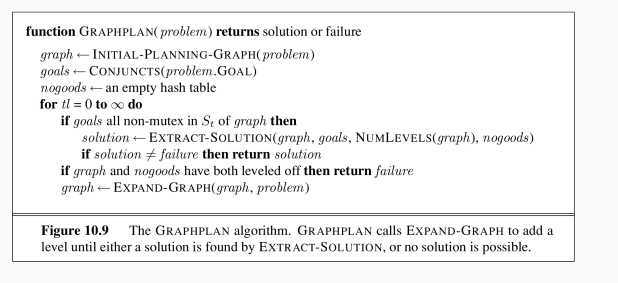
\includegraphics[scale=0.55]{01/graphplan.png}
    \caption{Algoritmo di Graphplan.}
\end{figure}

\dfn{Extract Solution}{
  L'estrazione di un piano da un grafo di pianificazione corrisponde a una ricerca backward in un sottografo AND/OR del GP:
  \begin{itemize}
    \item OR: gli archi che dalle aziono a un livello $A_{i-1}$ producono un letterale $p$ in un goal $g$ al livello $S_i$. 
    \item AND: sono gli archi che dagli atomi a un livello $S_i$ rappresentano le precondizioni per un'azione al livello $A_i$.
  \end{itemize}
}

\clm{}{}{
  \begin{itemize}
    \item Si sfrutta una funzione di supporto \texttt{GP-Search}. Sono \fancyglitter{mutuamente ricorsive}.
    \item \texttt{extract-solution} invoca \texttt{GP-Search} su un livello di azioni e su un sottogoal. 
    \item \texttt{GP-Search} pianifica per il solo livello su cui è invocato e se ha sucesso invoca \texttt{extract-solution} sul livello di stato precedente.
  \end{itemize}
}

\begin{figure}[h]
    \centering
    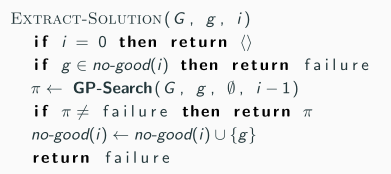
\includegraphics[scale=0.55]{01/extract.png}
    \caption{Extract-solution.}
\end{figure}

\begin{itemize}
  \item $G$ è il grafo di pianificazione. 
  \item $g$ è il sottogoal su cui la funzione è invocata. 
  \item $i$ è la profondità di un livello di stato $S_i$. 
\end{itemize}

\begin{figure}[h]
    \centering
    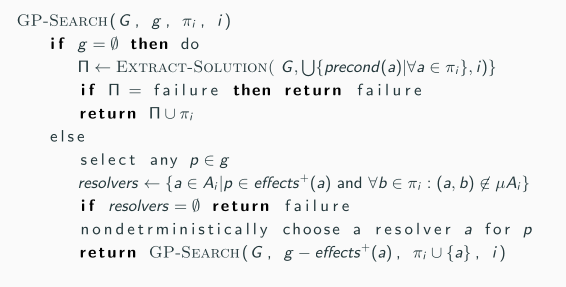
\includegraphics[scale=0.55]{01/search.png}
    \caption{GP-Search.}
\end{figure}

\begin{itemize}
  \item $G$ è il grafo di pianificazione. 
  \item $g$ è l'insieme di sottogoal ancora da risolvere al livello $i$. 
  \item $\pi_i$ è il piano in costruzione al livello $i$.
  \item $\mu A_i$ contiene le coppie di azioni al livello $i$ tra le quali sussiste un vincolo di mutua esclusione.
\end{itemize}

\paragraph{Considerazioni su \texttt{extract-solution}:}

\begin{itemize}
  \item È un algoritmo backward di ricerca all'interno di un grafo di pianificazione. 
  \item In generale questa ricerca potrebbe essere intrattabile e si ricorre quindi all'uso di euristiche. 
  \item Un modo semplice per implementare questa funzione  è un algoritmo greedy:
    \begin{itemize}
      \item Dato un insieme di letterali che compaiono nel goal scegliere il letterale con il costo di livello più alto. 
      \item Soddisfare il letterale scegliendo l'azione con le precondizioni più facili.
    \end{itemize}
  \item Ogni volta che \texttt{extract-solution} applicata a certi letterali $L$ e a un certo livello $lev$ fallisce la coppia $(L, lev)$ viene aggiunta nell'insieme $no-good$, per cui ricerche successive applicate alla stessa coppia falliranno immediatamente.
\end{itemize}

\nt{L'espansione del GP non si interrompe anche quando un grafo si è livellato. Un livello di stato può essere il risultato dell'applicazione di più azioni in parallelo. Quando l'esecuzione è sequenziale l'applicazione multipla di azioni riduce la dimensione del grafo che deve quindi essere esteso.}

\dfn{Terminazione di GP}{
  Se \texttt{extract-solution} non trova una soluzione deve esistere un sottoinsieme di atomi del goal che non sono raggiungibili vengono marcati come $no-good$  al livello successivo e quindi si continua a espandere. 

  Altrimenti quando sia il grafo sia i $no-good$ si sono livellati senza che una soluzione sia stata trovata si può concludere con fallimento.
}

\nt{Per far valere questo criterio bisogna dimostrare che: 
\begin{itemize}
  \item I $no-good$ si livellano sempre. 
  \item Quando i $no-good$ e il grafo sono livellati allora si può concludere che la soluzione non esiste.
\end{itemize}
}

\paragraph{La dimostrazione si basa su proprietà \fancyglitter{monotone} dei grafi di pianificazione:}

\begin{itemize}
  \item I letterali crescono monotonicamente: una volta che un letterale compare in un livello sarà presente in tutti i livelli successivi. 
  \item Le azioni crescono monotonicamente: una volta che un'azione compare in un livello sarà presente in tutti i livelli successivi.
  \item Le relazioni di mutex decrescono monotonicamente: se due azioni/letterali sono in mutua esclusione in un livello allora lo sono anche in tutti i livelli precedenti, ma potrebbero non esserlo in livelli successivi. 
  \item I $no-goods$ decrescono monotonicamente: se un sottoinsieme di atomi del goal non è raggiungibile in un dato livello di stato $S_i$ allora non lo è nemmeno in nessuno dei livelli precedenti, però potra diventarlo in qualche livello futuro. 
\end{itemize}

\paragraph{Dimostrazione che il grafo e i $no-goods$ si livellano e criterio di temrminazione:}

\begin{enumerate}
  \item Dato che le azioni e i letterali crescono monotonicamente, e dato che sono entrambi insiemi finiti, deve esistere un livello in cui l’insieme dei letterali è uguale a quello dei letterali del livello precedente. 
  \item Poiché i mutex e $no-goods$ decrescono monotonicamente e poiché non possono esserci meno di zero mutex e $no-goods$, deve esistere un livello con lo stesso numero di mutex e $no-goods$ del precedente. 
  \item Una volta che il grafo ha raggiunto la situazione in cui sia i livelli che i $no-goods$ si sono livellati, se uno dei letterali del goal è mancante o in mutex con un altro letterale del goal, allora si può concludere che non esiste una soluzione.
\end{enumerate}

\nt{Graphplan è \fancyglitter{corretto} e \fancyglitter{completo}: restituisce failure solo quando il problema di pianificazione non è risolubile, altrimenti restituisce una soluzione espressa  come una sequenza di insiemi logici di azioni. L'algoritmo termina sempre a prescindere dall'esistenza della soluzione.}

\subsection{Definire Euristiche}

\dfn{Rilassamento}{
  Si definisce un problema analogo all'originale, ma rilassato (semplificato). Si risolve il problema rilassato e si usa il costo della soluzione per il problema rilassato come euristica nel problema originale.
}

\paragraph{Possibili tecniche di rilassamento di un problema:}

\begin{itemize}
  \item \fancyglitter{Delete relaxation:} cancellazione degli effetti negativi dalle azioni. 
  \item \fancyglitter{Astrazione:} considerare un problema più piccolo, ignorare alcune differenze tra stati così che  collassino in un unico stato (spazio di ricerca ridotto). 
  \item \fancyglitter{Landmark:} un insieme di azioni (o fatti) per cui ogni soluzione deve avere almeno un'azione di quest'insieme, sono usati per definire euristiche che fanno un safe pruning dello spazio di ricerca.
\end{itemize}

